\chapter{Introduction}
\label{sec:introduction}
%\chapter{Einleitung}
%\label{sec:einleitung}
Unmanned Aerial Vehicles, both fixed and rotory winged, have found plathora of applications in a wide variety of fields in recent years. Precision agriculture, environmental and  wildlife monitoring, search and rescue missions are but a few examples where UAVs are already making a visible impact. A more denser and seemless integration of unmanned aerial vehicles, especially autonomous unmanned aerial vehicles flying beyond line of sight, in day to day life poses a variety of challanges, both social and scientific. On the technical side, it requires UAVs to have a better, more richer understanding of the environmemnt they operate in. Apart from developing a higher level of cognitive understanding of the UAV's surroundings, still an open research problem, it is vitally important for the UAV to be able to create a simplified map of it's surroundings and use it for navigate across obstacles and avoid collisions. Thus, Simultaneous Localization and Mapping for autonomous unmanned aerial vehicles flying in unknown environments has garnered a lot of research interest. The ability to create a map of a UAV's surrounding environment in realtime using onboard sensors and estimate it's location in relation to the map enables the possibility of online path planning for collision avoidance in unknown environments.\\
At the top level, it is this problem of building a map of a fixed winged UAV's immediate surroundings and localizing the UAV within the map, onboard and in realtime, for the purpose of navigation and collision avoidance is what is delt with in this semester thesis. In the following sections, the specific SLAM problem being tackled in the thesis is motivated and the system's specifications are described, followed by problem formulation and an outline of the solution approach.



\section{Motivation}
\label{sec:intro_motivation}
Fixed wing UAVs are more efficient in forward flight than their rotary wing conterparts, having to spend energy only to counter the aerodynamic drag(in addition to powering electronics) and using aerodynamic lift to balance weight, in contrast to rotary wing UAVs that spend energy to counter both weight and drag. This makes fixed wing UAVs ideally suited for long range or high endurance missions such as search and rescue operations in outdoor environments. The requirement to operate autonomously or semiautonomously in such unknown or unmapped terrains for these missions makes onboard mapping a necessity for safe and reliable operation. Of the variety of information rich onboard extereoceptive sensors that have been studied for their application in SLAM, including range sensors like Laser scanners and vision sensors like RGB-D cameras, stereo and monocular cameras, the payload's weight and energy constraints on small UAVs poses significant restrictions on the kind of sensors that can be used on such small airborn vehicles.\\ 
Compact, light weight and low cost sensors like monocular cameras providing information rich snapshots of the surroundings deliver many advantages from the point of view of UAV's payload and energy requirements. At the same time, they also pose significant challanges in terms of their application for SLAM. Unlike range sensors like laser scanners, monocular vision sensors do not provide direct measurements of the 3D coordinates of the terrain, but require it to be extracted from the sequence of images they provide. Similarly, while laser range sensors and both RGB-D cameras and stereo vision sensors can make measurements with an associated metric scale, scale by itself is not observable in measurements made by a monocular vision sensor. That is, camera translation and scene depth can both be changed such that the measurements made by the monocular camera remains constant. This requires the fusion of sensor measurements made by some other mertic sensor onboard the aircraft with the measurements from the monocular camera to both counter scale drift and recover the global scale and orientation of the map.\\
Since the purpose of mapping is to enable a path planning procedure for collision avoidance, building and maintaining a map only of the UAV's local surroundings is deemed sufficient, rather than maintaining a map over the entire history of the UAV's mission, in light of the expected long range and exploratory nature of the mission and limited computational capabilities of the onboard computer. This motivates the semster thesis to deal with real-time mapping over a sliding window on a fixed wing UAV for the purpose of navigation and collision avoidance using a monocular vision sensor. Details of the aircraft, it's various sensors and the flight mission are described in the following section.

\section{System Description}
\label{sec:intro_sys_description}
The onboard reconstruction pipeline built over the course of the semester project was targeted to be used aboard the AtlantikSolar fixed wing aircraft. The aircraft was built as a part of the AtlantikSolar project\cite{atlanticSolar} of the aerial vehicles group at the Autonomous Systems Lab (ASL) of ETH Zurich. The project aims to fly a solar powered fixed wing aircraft across the atlantic ocean. The aircraft itself is a 5m-class solar powered fixed wing UAV that is designed for minimal power consumption and high flight efficiency. Figure \ref{pic:atlantic_solar_basic} shows the aircraft in flight and Table \ref{tab:atl_sol_specs} gives the system's technical specifications.
% \usepackage{graphics} is needed for \includegraphics
\begin{figure}[htp]
\begin{center}
  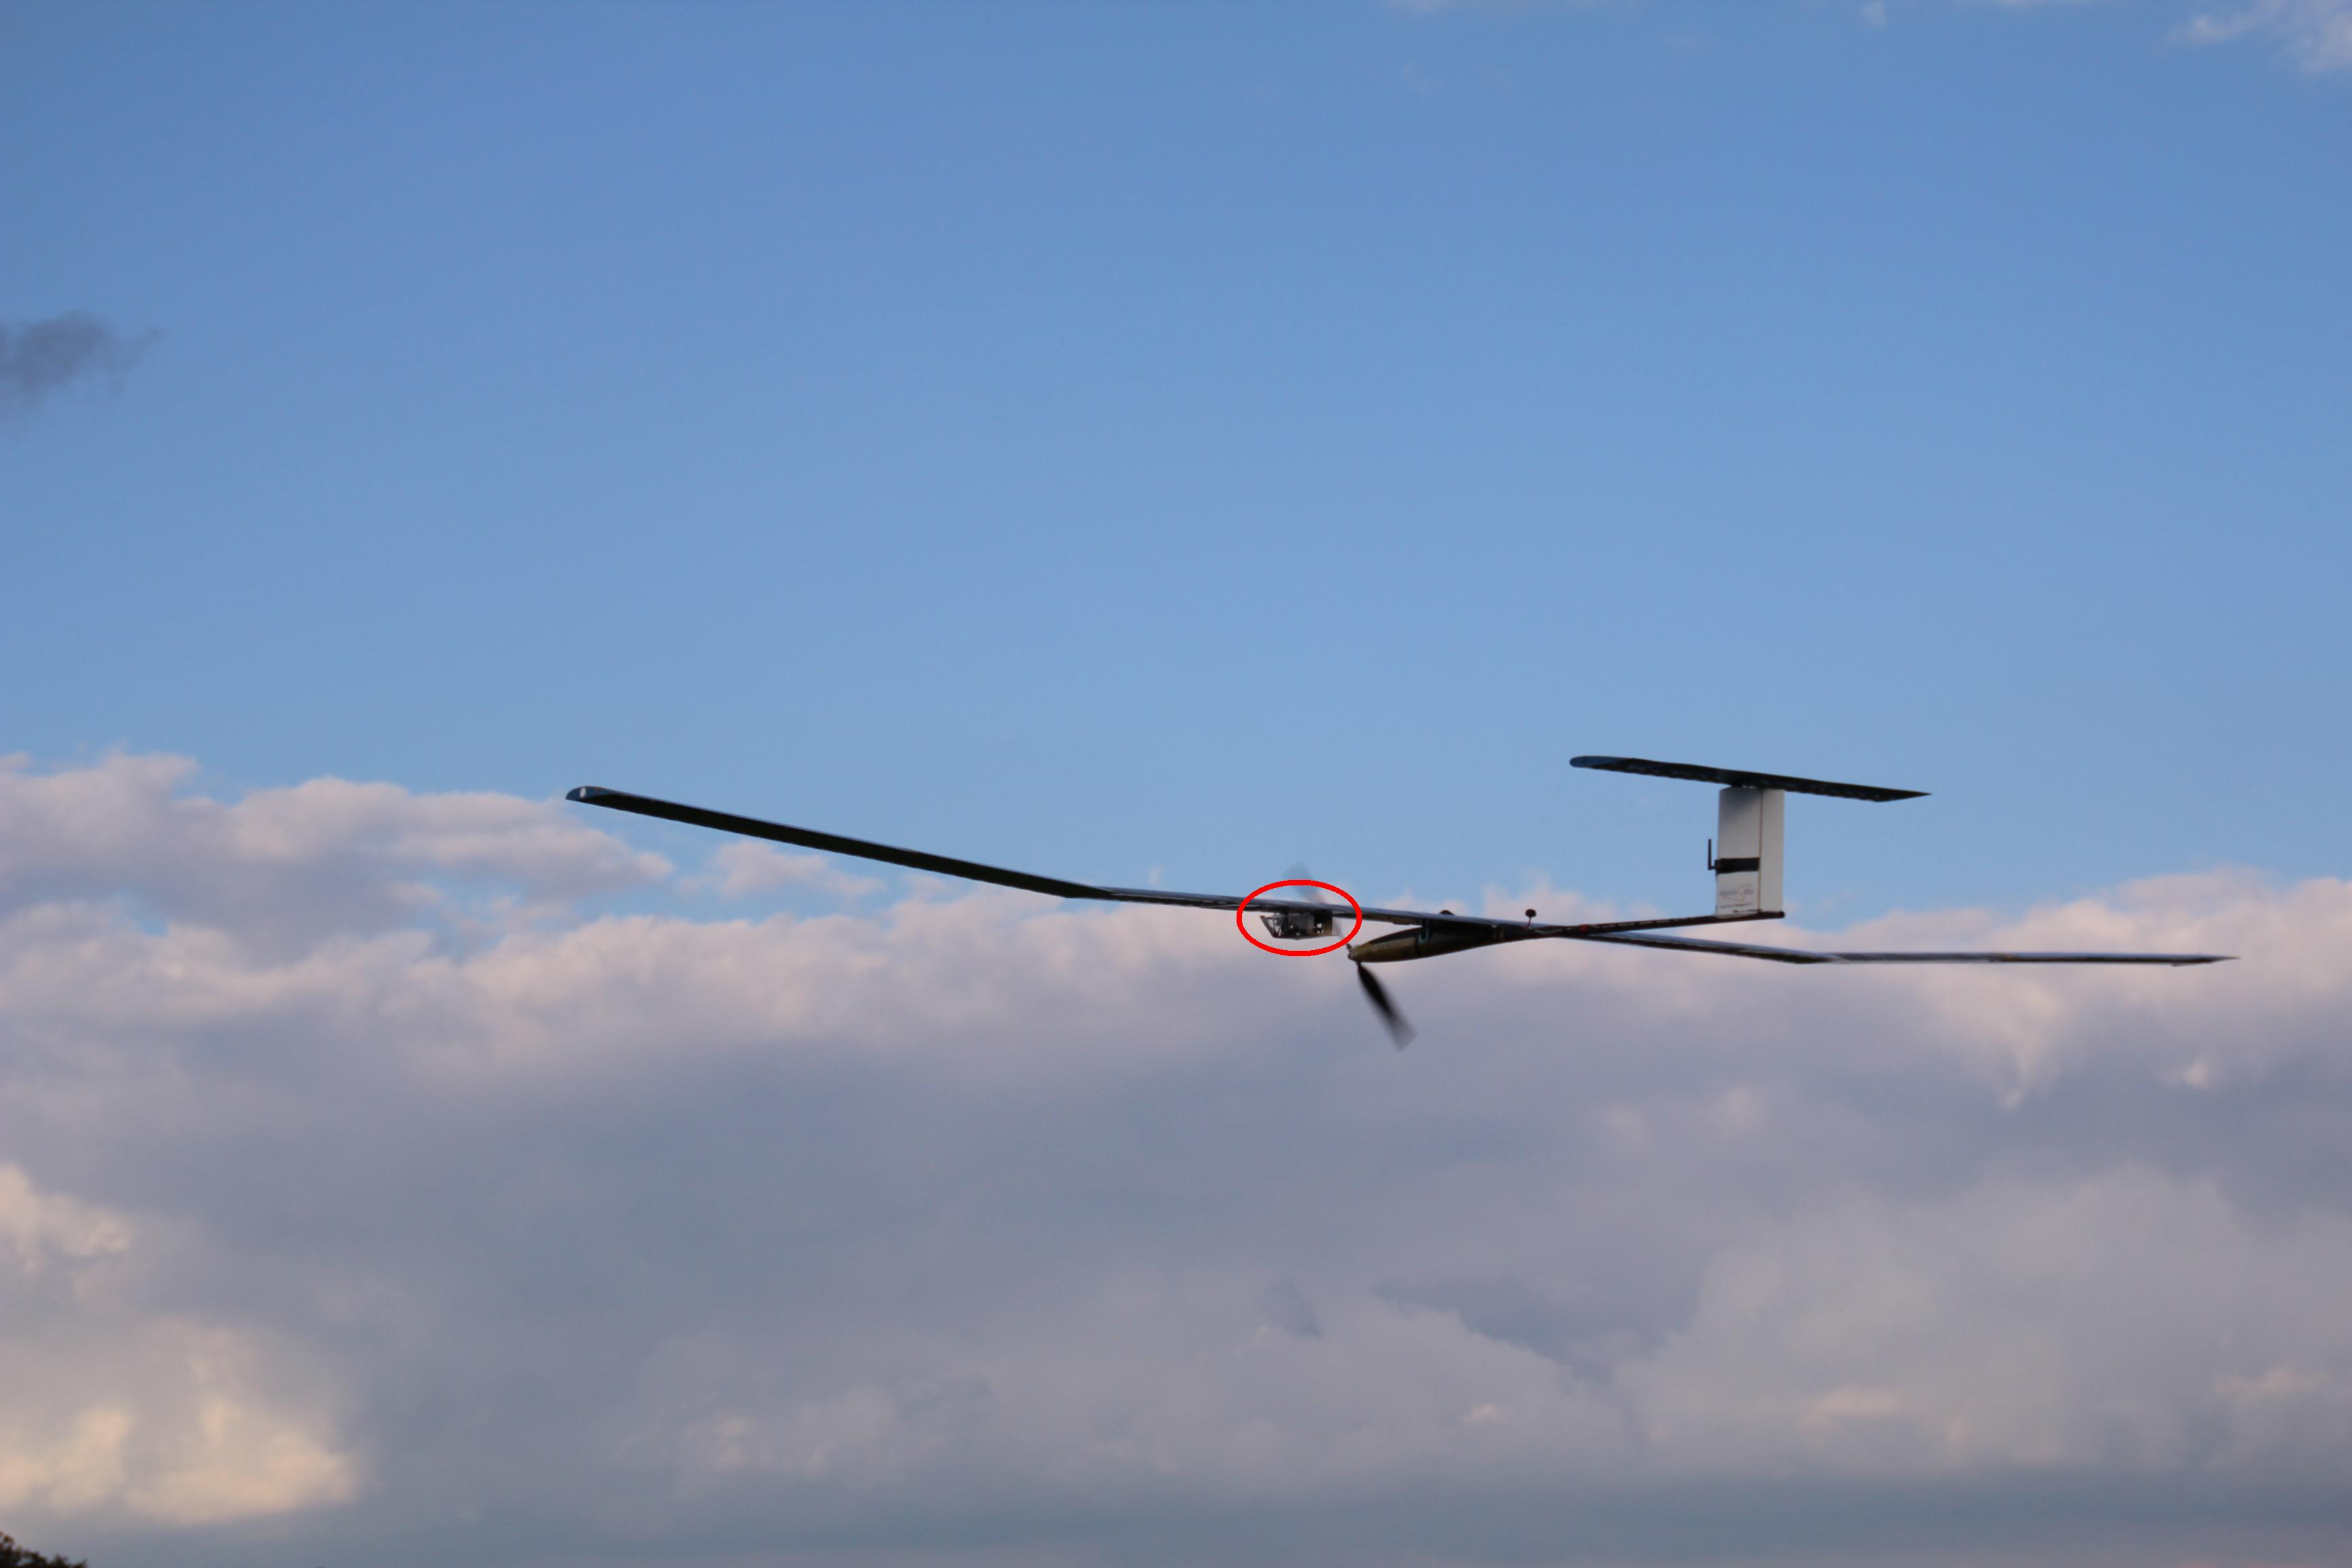
\includegraphics[width=\textwidth]{images/atlantic_solar}
  \caption{AtlantikSolar fixed wing UAV, vision sensor shown in red oval.}
  \label{pic:atlantic_solar_basic}
\end{center}
\end{figure}

\begin{table}%{l}{0.4\textwidth}
\vspace{-10pt}
\centering
\caption{Atlantic Solar aircraft Specifications}
\begin{tabu} to 0.4\textwidth {l|r}
\textbf{Specification} & \textbf{Value} \\ \hline
Mass & 6.2 kg \\
Span & 5.6 m \\
Cruise velocity & 9.5 m$s^{-1}$\\
Cruise flight altitude & $\sim$400 m above sea level\\
Structure & Light weight carbon fiber and kevlar\\ \hline
Camera Sensor & Monocular camera, Aptina MT9V034 sensor\\
FOV & 60/100 degrees \\
Camera mount location & Wing, 60 cm from fuselage \\
\bottomrule
\end{tabu}
\label{tab:atl_sol_specs}
\end{table}

The aircraft features a multisensor fusion EKF based state estimator as described by Stefan \cite{6981466} using measurements from onboard IMU, static and dynamic pressure sensors, compass and GPS. The estimator provids position, velocity, attitude and heading estimates. It also gives unbiased estimates of attitude, airspeed and AoA in case of GPS outages.\\
The monocular vision sensor is mounted on the wing of the aircraft looking ahead in the direction of motion with it's principle axis pointing about half way below the aircraft nose axis to it's body z axis (body yaw axis). The sensor mount location is about 60 cm away from the fuselage on the wing, as shown in red in Figure \ref{pic:atlantic_solar_basic}. Although the structure of the aircraft is rigid, mounting of the sensor away from the COG leads to low amplitude high frequency oscillations from the dynamic modes of the structure and excitations from propeller. These oscillations have not been measured, but the presence of this phenomena has been verified through an inflight onboard FPV camera. This leads to there being a non-rigid link between the inertial measurement unit mounted close to the COG and the monocular sensor mounted on the wing. Thus, fusing the inertial measurement sensor data together with the monocular vision sensor data, as is often done, would require complex online calibration of the non-rigid link which was deemed outside the scope of this semester project.\\
The datasets used for the semester thesis were obtained through Atlantic Solar's flight over Marche-en-Famenne, Belgium at an altitude of $\sim$80 m above ground as a part of ICRAUS field trials. An example of the kind of scenary and the type of image acquired by the monocular vison sensor can be seen in Figure \ref{pic:sensor_image}\\

% \usepackage{graphics} is needed for \includegraphics
\begin{figure}[htp]
\begin{center}
  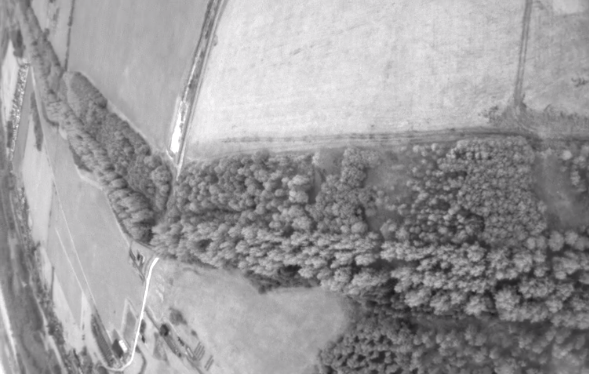
\includegraphics[width=\textwidth]{images/sensor_image}
  \caption{Image aquired from monocular vision sensor at altitude $\sim$80 m.}
  \label{pic:sensor_image}
\end{center}
\end{figure}


\section{Problem Statement}
\label{sec:intro_prob_statement}
Given the motivation of the project as described in section \ref{sec:intro_motivation} and the system as described in section \ref{sec:intro_sys_description}, it was decided to create an onboard reconstruction pipeline mapping over a sliding window for fixed winged aircraft using monocular vision for the purpose of collision avoidance. The inputs available to the system were the image sequence obtained from the monocular vision sensor and the GPS data. The expected output was a pointcloud in global frame which could be meshed for the purpose of path planning.


\section{Solution Approach}
\label{sec:intro_sol_approach}
Using inertial measurement data and vision sensor data in a complementary manner through a sensor fusion framework for SLAM in a loosely-coupled\cite{6225147} or tightly-coupled\cite{Leutenegger-RSS-13} fashion has long been popular in the robotics community\cite{Hesch_towardsconsistent}. Due to the presence of a non-rigid link between the inertial measurement unit used in the UAV's state estimator and the monocular vision sensor as described in section \ref{sec:intro_sys_description}, such an approach would require an online estimation of the dynamics of the non-rigid link, to enable effective fusion of inertial measurement data with the vision sensor data. This approach would entail a deep integration of the vision sensor data, and states representing the dynamic motion of the non-rigid link, into the state-estimator \cite{6981466} already running on the onboard controller. This would enable the entire UAV to have a unique state estimator utilizing all available sensors at the cost of increased complexity. In contrast to this approach, running a visual-slam algorithm as a standalone addon to the system for the explicit purpose of mapping and path-planning, and not for low-level control, would create a loosely coupled system where the coupling between the low level controller and the visual based localizer and mapper would arise solely through the path-planner. This would lead to reduced complexity and generalized pipeline that could work even in the absence of an IMU at the cost of almost total reliance on visual measurement and, possibly reduced robustness to rapid manoeuvers(causing motion blur or degenerate motions like pure rotation) due to discarding the additional benefits of inertial measurements.\\
Since the mapper for path-planning was deemed not as flight critical as, for example, a low level controller, it was decided to go for the loosely coupled approach of using monocular vision SLAM (aided by GPS to recover metric scale and global orientation) instead of the former approach of deep integration of vision sensor data in the state estimator and estimating the dynamics of the non-rigid link.\\
For the purpose of vision based localization and mapping, feature point based parallel tracking and mapping package PTAM\cite{Klein:2007:PTM:1514339.1514363} and direct image alignment based Large Scale Direct monocular SLAM package LSD-SLAM\cite{engel14eccv} were considered. In our brief trials with PTAM, it was observed that the point features were not being tracked over many frames as the limited field of view of the camera coupled with large altitude and rotations led to rapid change of observed scenary causing repeated tracking loss and reinitializations. Initialization procedure for PATM also posed restriction on aircraft motion(requiring smooth translation) without which inflight initialization often localized an incorrect plane as the ground plane. Apart from this, the large scale outdoor exploratory nature of our mapping requirements was different from scene generally used with PTAM, i.e. moving in and around a small workspace\cite{Klein:2007:PTM:1514339.1514363}.\\
In contrast to this, LSD-SLAM is much more suitable for our mission as it is designed for large scale mapping, and provides both visual odometry and semi-dense depth maps that can directly be used for path planning (not requiring a separate dense reconstruction pipeline for sparse feature point maps populated by most feature based slam algorithms). After obtaining encouraging initial results with LSD-SLAM, it was decided to go forward with it. Apart from this, since monocular vison by itself cannot observe either the metric scale or the global pose of the map, which were necessary for using the map in path planning, the integration of GPS measurements into the vision slam through the LSD SLAM's pose graph framework was thought suitable. It was also decided to switch from g2o\cite{5979949} already integrated in LSD-SLAM's software architecture to GTSAM\cite{gtsam} for graph optimization as it provided fixed lag smoothing that would be required to implement marginalization of previous measurements and maintaining a map only over a sliding window.

